\documentclass{report}

\usepackage[english]{babel}

\usepackage[letterpaper,top=1.8cm,bottom=2cm,left=2cm,right=2cm,marginparwidth=1.6cm]{geometry}

\usepackage{enumitem}
\usepackage{multicol}
\usepackage{titlesec}
\usepackage[T2A]{fontenc}
\usepackage[utf8]{inputenc}
\usepackage{graphicx}

\graphicspath{ {./images/} }

\begin{document}

\renewcommand{\baselinestretch}{0.9}
\renewcommand{\thesection}{\Roman{section}}
\titleformat{\section}{\footnotesize\centering}{\thesection. }{0cm}{}[]

\setcounter{page}{177}
\setcounter{section}{4}

\begin{center}
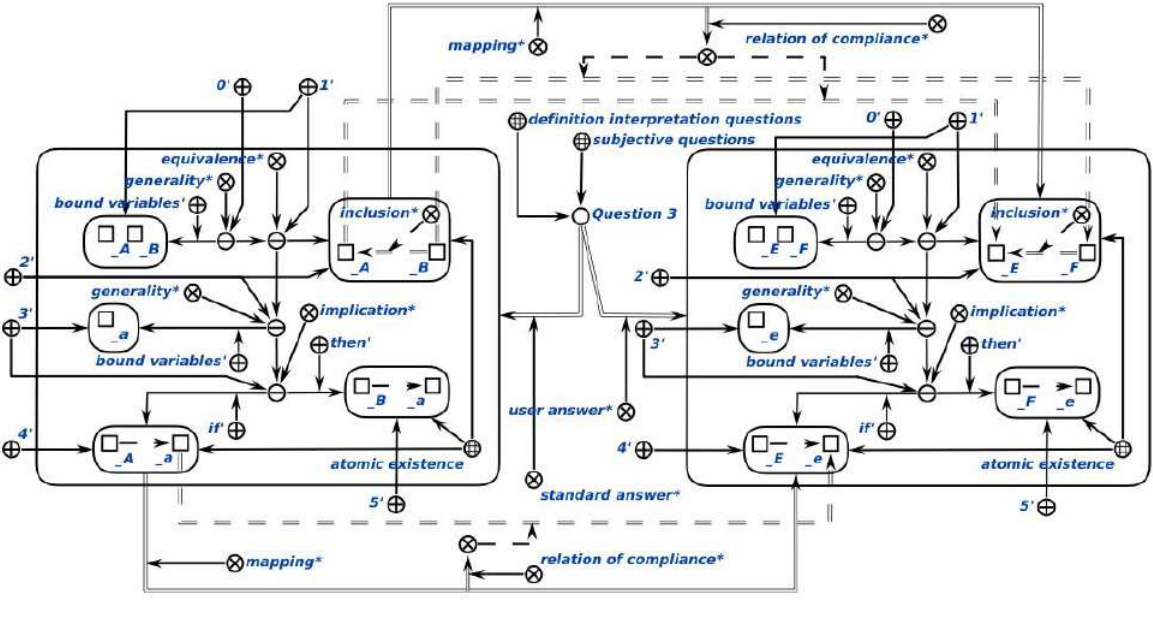
\includegraphics[width=17cm, height = 9cm]{1.png}
\parbox[c]{16.4cm}{\scriptsize{Figure 3.~} An example of establishing the mapping relationship of potential equivalent variable sc-node pairs between semantic graphs }
\vspace{1mm}
\end{center}

\begin{small}

\begin{multicols}{2}

\setlist{nolistsep}

\begin{enumerate}
\item [] user answer are numbered respectively, and the mapping
relationship of potential equivalent variable sc-node pairs
between answers is established;
\item [5)]iteratively traverse each substructure of the standard
answer and user answer, classify them according to
the type of substructure, and count the number of all
substructures;
\item [6)]one type of substructure is randomly selected from the
set of recorded standard answer substructure types;
\item [7)]according to the standard answer substructure type selected in step 6), a corresponding type of substructure is
selected from the set of recorded user answer substructure types;
\item [8)] iteratively compare each substructure with the same substructure type between the standard answer and the user
answer, and record the number of matched substructures
and the matched substructures.
\item [9)]repeat step 6 — step 8 until all types of substructures
have been traversed;
\item [10)] using formulas (1), (2), (3) calculate precision, recall and
similarity, and generate semantic fragments for recording
sc-agent running results;
\item [11)] removing all temporary sc-elements created while the
sc-agent is running;
\item [12)] exit the program.
\end{enumerate} 

\par When the precision, recall and similarity between the answers to the subjective questions are obtained, the completeness
and correctness of the user answers can be evaluated. According
to the similarity, user answers are divided into the following
situations:

\begin{itemize}
    \item[$\bullet$] if the similarity is equal to 1, the user answer is completely correct ($F_{sc}$ = 1);
    \item[$\bullet$] if the similarity is greater than 0 and less than 1 (0 < $F_{sc}$ < 1), there may be two situations:
    \begin{itemize}
        \item [\textbf{--}] the user answer is partially correct and incomplete (the default mode of the current version);
        \columnbreak
        \item [\textbf{--}] the logical formulas used to formalize standard answers and user answers may satisfy logical equivalence (in the following article, we will introduce in detail the approach to judging the equivalence between answers based on predicate logic).
    \end{itemize}
    \item[$\bullet$] if the similarity is equal to 0 ($F_{sc}$ = 0), the user answer is completely wrong.
\end{itemize}
\section{CONCLUSION AND FURTHER WORK}
\hspace{\parindent}Automatic answer verification is one of the most basic functions of ITS, which can quickly check the user mastery of new
knowledge and improve the user learning efficiency. Therefore,
this article introduces in detail an approach to developing a
problem solver for automatic answer verification in the ITS
developed using OSTIS Technology. The developed problem
solver can not only verify the correctness and completeness of
the answer to the subjective question, but also the correctness
and completeness of the answer to the objective question.
Because the problem solver is developed based on multiagent technology, sc-agent for computing semantic similarity
of factual knowledge, sc-agent for processing semantic similarity calculation results of factual knowledge, and sc-agent
for computing semantic similarity of logical knowledge are
developed in this article respectively. The developed problem
solver completes the answer verification by combining different
sc-agents according to the type of the question.
\par The developed problem solver for automatic answer verification in this article has the following advantages:

\begin{itemize}
  \item[$\bullet$] verify the correctness and completeness of user answers
  based on semantics;
  \item[$\bullet$] by calling different sc-agents, the similarity between any
  two semantic fragments in the knowledge base can be
  calculated;
  \item[$\bullet$] because the problem solver is developed based on multiagent technology, it is easy to add new functions;
  \item[$\bullet$] because the ostis-systems developed for different application fields have the same knowledge representation
  \end{itemize}

\end{multicols}

\end{small}

\end{document}
